
\documentclass[12pt, letterpaper]{article}
\usepackage[utf8]{inputenc}
\usepackage{pgfplots}
\usepackage{subcaption}
\usepackage{graphicx}
\usepackage{float}
\usepackage[english,main=russian]{babel}
\usepackage[T1]{fontenc}
\usepackage[backend=biber,style=numeric,sorting=none]{biblatex}
\usepackage{todonotes}
\addbibresource{FatigueDetector.bib}
\graphicspath{{src/Images/}} 


\title{Определение степени усталости человека по фотографии}
\date{\today}
\author{Муртазин Виталий, Фасхутдинов Тимур, \and
Тимергалин Денис, Ямиков Рустем, \and
Байрамов Азат, Саяхов Ильфат, Туманов Никита
}

\begin{document}

    \maketitle

    \begin{abstract}
        В этой статье будут описаны решения проблемы распознавания усталости человека по изображению его лица.
        В ходе данной работы сначала будут рассмотрены уже существующие алгоритмы.
        Затем будет предложена и реализована модель собственной архитектуры.
        В заключении будут приведены итоговые показатели работы модели.
    \end{abstract}

    \section{Вступление}\label{sec:introduction}
    В книге Хуллермайера Э. и Рифки М. дается определение: <<Психическая усталость представляет собой психобиологическое состояние, вызванное длительными периодами вынужденной умственной активности, и имеет последствия для многих аспектов повседневной жизни>>\cite{hullermeier_fuzzy_2009}.
    Было обнаружено, что на рабочем месте умственная усталость приводит к повышению риска ошибки \cite{__nodate}.
    Такие ошибки могут привести к снижению производительности на рабочем месте, а также трагическим последствиям.

    Одна из отраслей, в которой влияние усталости на безопасность уже давно признано - это транспорт.\cite{phillips_fatigue_2017}.
    
    "По оценке национального управления безопасности дорожного движения США минимум 100 000 аварий ежегодно происходят из-за усталости водителя, в которых погибает около 1550 человек, получают ранения 71 000 человек"\cite{qiang_ji_real-time_2004}.

    В Российской Федерации по данным статистики за 2017 год зарегистрировано около 126 000 дорожно-транспортных происшествий, в которых каждое пятое возникает по причине усталости, а среди ДТП со смертельным исходом - каждое четвертое \cite{__2018}.

    Исходя из вышеперечисленной статистики можно сделать вывод, что проблема усталости человека на рабочем месте актуальна на данный момент и требует решения.
    Результат исследования позволит снизить риск несчастных случаев по причине утомления работника.

    Для определения усталости существует множество признаков и некоторые из них можно выявлять при помощи камеры \cite{singh_monitoring_1999}.
    На текущий момент методы распознавания лиц развиваются и используются в различных областях человеческой деятельности, включая обнаружение глаз при анализе лиц, отслеживание взгляда и т.д.
    Как правило, на первом этапе определяется местоположение лица, затем выделяются черты лица с очевидными краями, например, контуры глаз \cite{wen-bing_horng_driver_2004}.

    Целью данного исследования является создание программного продукта, определяющего усталость человека по фотографии с использованием сверточных нейронных сетей.
    Объектом исследования является детектирование признаков усталости (определение степени усталости) человека на рабочем месте.

    \section{Проблема}\label{sec:problem}

    В современном мире актуальна проблема повышенной утомляемости людей из-за чрезмерной нагрузки,
    a чем выше усталость человека, тем выше вероятность ошибки.
    В некоторых сферах цена ошибки очень высока.
    Она может привести к убыткам, а в худшем случае может нанести ущерб здоровью.

    К личностным (психофизиологическим) причинам производственного травматизма условно можно отнести физические и нервно-психологические перегрузки работника, приводящие к его ошибочным действиям. Из-за утомления, вызванного большими физическими и умственными перегрузками у человека уменьшается бдительность, что может привести к печальным последствиям не только на рабочем месте, но и после работы, например по пути после работы \cite{noauthor__nodate-1}.

    Экспериментально доказано, что все аварии и несчастные случаи коррелирует с наступлением усталости,
    a средством противодействия развития усталости выступает фактор заинтересованности в работе.
    Поэтому можно утверждать, что на склонность к несчастным случаям влияет также уровень заинтересованности и удовлетворенности человека своей работой \cite{noauthor__nodate-2}.

    Усталость ведет к потере внимания и концентрации.
    Кроме того, уставший человек невольно пытается закончить порученную ему работу как можно быстрее, что в умножении на нашу привычку работать в режиме аврала, приводит к плачевным последствиям \cite{noauthor__nodate-4}.

    Но, к сожалению, рабочие места не всегда соответствуют требованиям законодательства.
    Кроме того, работник может получить травму в результате причин субъективного характера.
    Например, усталость, головокружение, невнимательность, нестабильный эмоциональный фон — все эти причины могут быть источником производственной травмы \cite{noauthor__nodate-3}.

    В небезопасной рабочей среде и при комбинации названных факторов вопрос не в том, произойдет ли на работе несчастный случай, а в том, как скоро он произойдет \cite{evijafeierabende__2017}.

    Однако если вовремя определять усталость людей и не допускать их до рабочего процесса, то можно минимизировать последствия ошибок.

 \section{Обзор существующих решений}\label{sec:approaches-review}
 
    Множество готовых решений существует в автомобилестроении. Многие компании-производители встраивают в свои автомобили системы определения усталости. Например, в некоторых моделях Toyota с 2008 года используется технология распознавания усталости по положению век.
    
    Другое решение используется в автомобилях Nissan: там система запоминает паттерн движения руля водителя в активном состоянии и сигнализирует об усталости, если обнаруживает отклонения от существующего паттерна.
    
    Ещё одно решение было предложено компанией Volkswagen. Их автомобили так же отслеживают поведение руля, но кроме этого они используют системы наблюдения за нажатием педалей и систему слежения за полосой движения.\cite{sikander_driver_2019}
    
    Так же мы рассмотрели и изучили систему распознавания усталости под названием - "Perclos". Данная система работает с веками человека, реагируя на их закрытие над зрачком с течением времени, с какой скоростью они закрываются и открываются. Очень многие производители автомобилей используют данную систему, но не только, как уникальную разработку, а интегрируют собственное программное обеспечение на основе данной технологии.
    
    На первый взгляд, данное решение очень подходит для определения усталости, но в ходе исследования данной технологии мы выяснили, что у этой системы есть ряд недостатков. 

    Во-первых внешние факторы - пыль, недостаточное освещение, блики и перепады влажности. Все это, а также индивидуальное поведение глаз отдельного индивидуума может вызвать ошибочные результаты. Так же для нашего решения определения усталости система ``Perclos`` не подходит, так как данная технология определяет усталость в режиме реального времени, а мы решаем проблему с определением усталости в начале рабочего процесса. \cite{david_f_dinges_perclos_nodate}
    
    Для распознавания усталости используется множество различных техник машинного обучения, которые обладают своими специфичными особенностями, преимуществами и недостатками. Достаточно полно их специфика применения была рассмотрена в статье \cite{yadav_survey_2020}, где был осуществлен обзор основных 8 способов машинного обучения, применяемых для детектирования усталости:
    \begin{enumerate} 
        \item Методы на основе локальных бинарных шаблонов отличаются высокой эффективностью вычисления, однако автоматическая локализация лица может обладать недостаточной точностью.
        \item Схожим недостатком обладает и метод обнаружения краев Собеля, который определяет область лица целиком, с дальнейшим выделением границ глаз. Способ позволяет идентифицировать края и их ориентации, однако невозможно добиться точного распознавания краев, а работа алгоритма требует длительного времени.
        \item Следующий рассмотренный в статье\cite{yadav_survey_2020} способ - это использование признаков Хаара для обнаружения лица,  с дальнейшим извлечением признаков глаз. Методика обладает высокой скоростью вычисления, также имеет высокую точность обнаружения и может позволить получить точный результат даже на засвеченном изображении. Главным недостатком является очень длительное время обучения.
        \item Статическая Байесовская сеть использует для прогнозирования такие особенности, как движение глаз, движение головы, выражение лица и т.д. Достоинство метода заключается в том, что обладает сходимостью сложности задачи, однако недостаток в том, что автоматическое решение все равно вычислительно невыполнимо из-за огромного объема необходимых вычислений.
        \item Техника оценивания взгляда обнаруживает зрачок глаза на основе извлечения таких признаков как корень носа, кончик носа, нижняя часть лица, правый глаз, левый глаз. Состоит из стадий распознавания зрачка, отслеживание взгляда, калибровка и установление его расположения. Отслеживание взгляда становится все более точным по мере построения большего количества выравненных фокусов. Однако отслеживание взгляда зависит от используемой методики точной корректировки.
        \item Нечеткая экспертная система позволяет определить усталость по выражениям лица, например движению глаз, закрытию глаз, зевоте. Техника имеет быструю скорость выдачи ответа и малые вычислительные затраты. Главным ограничением является требования большого объема мета-знаний экспертом для составления нечетких правил.
        \item Анализ связанных компонент сосредоточен на извлечении признаков глаз. Определяет области глаз учитывая как локальную, так и глобальную информацию для сегментации, однако алгоритм работает в полуавтоматическом режиме, требуя пользовательского участия и экспертизы.
        \item Сверточные нейронные сети работают на основе таких признаков, как выражения лица, моргание, длительность закрытия глаз, зевота. Сети имеют высокую точность даже при проблемах с распознаванием изображений и способны к лучшей характеризации изображения. Среди недостатков CNN выделяют высокая стоимость вычисления и требование большего числа тренировочных данных.
    \end{enumerate}
    
\section{Архитектура}\label{sec:architecture}    
   
    Идея сверточных нейронных сетей (англ. CNN - convolutional neural networks) состоит в чередовании сверточных и субдискретизирующих слоев. Каждый сверточный слой состоит из нескольких наборов нейронов. Каждый набор отвечает за свою карту признака (англ. feature map) - матрицу состояний нейронов набора и координат. Все нейроны набора имеют общий вектор весов, а их рецепторные поля расположены в разных местах, позволяя детектировать конкретный признак по всему изображению. Эти признаки комбинируются и переиспользуются в следующих слоях. Для обучения используется алгоритм обратного распространения ошибок\cite{bengio_convolutional_1997}.

    \begin{figure}[H]
        \centering
        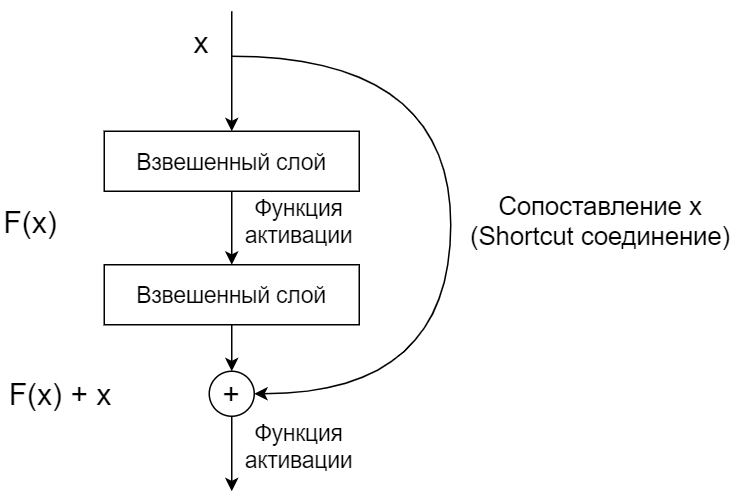
\includegraphics[width=0.7\linewidth]{ResNet_scheme.png}
        \caption{Блок с shortcut соединением в нейросети ResNet}
        \label{fig:ResNet_scheme}
    \end{figure}

    В данном проекте использовалась нейросеть ResNet-152v2\cite{he_deep_2015}. Особенностью этой модели нейросети являются, так называемые "соединения быстрого доступа" (shortcut connections), которые позволяют пропустить несколько слоев (Рис. \ref{fig:ResNet_scheme}). Таким образом, решается проблема других сверточных нейронных сетей, где с увеличением количества уровней точность сначала увеличивается, а затем начинает резко падать.
    
    В используемой нами нейросети ResNet-152v2 указали вводные данные, а именно - отключаем верхний уровень нейронной сети (include\_top = False), установили предварительное обучение в imageNet (weights = 'imagenet') и установили дополнительный режим объединения (устанавливается в том случае, если include\_top имеет значение False) - pooling = 'avg'. 
    avg означает, что глобальное среднее объединение будет применено к выходным данным последнего свёрточного блока, и, таким образом, выходом модели будет двухмерный тензор.
    Использовались функция потерь - категориальная перекрестная энтропия, алгоритм оптимизации Адам и функция активации softmax.
    
    В конечном решении использовался размеченный датасет <<fatigue detection>>\cite{noauthor_fatigue_detection_nodate}. Он включает в себя наборы фотографий людей для обучения, тестирования и использования нейросети. Каждый набор разделен на три класса: бодрствующий, невнимательный, уставший. Соответственно, программа решает задачу классификации для этих трех классов. Всего в датасете насчитывается около 4 тыс. фотографий людей с разным уровнем освещения, положением головы и направленностью взгляда.
    
    Вся разработка проводилась в Google Colaboratory\cite{noauthor_colaboratory_nodate}. Данный сервис был выбран из-за удобства совместной разработки и доступа к удаленным ресурсам, на которых запускается код.
    
    При разработке нейронной сети использовалась библиотека Keras\cite{noauthor_keras_nodate}. Keras — это открытая библиотека для машинного обучения, которая позволяет легко использовать фреймворк TensorFlow\cite{noauthor_tensorflow_nodate}. Она содержит в себе множество уже готовых нейронных сетей, в том числе и ResNet-152v2. Это очень облегчает процесс описания архитектуры нейронной сети.
    
    Так же использовалась библиотека dlib для предобработки входных данных (фотографий).
    Перед подачей изображения непосредственно на саму нейросеть изображение нормируется. На первом этапе при помощи метода <<get\_frontal\_face\_detector>> определяется расположение лица на фотографии, затем обрезается лишняя часть и масштабируется до 250 пикселей с каждой стороны.
    
    \begin{figure}[H]
        \centering
        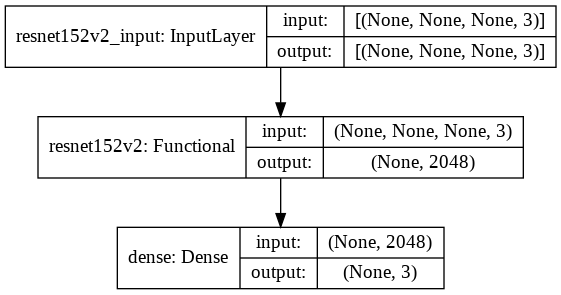
\includegraphics[width=1\linewidth]{model.png}
        \caption{Визуализация модели нейронной сети}
        \label{fig:model}
    \end{figure}
    
    Поверх нейронной сети ResNet-152v2 (Functional) были добавлены 2 слоя. InputLayer - он является входным слоем, который принимает данные о изображении. Его размерность составляет 250x250x3, что соответствует размеру изображения 250x250 и 3 для кодирования RGB цвета.
    И последний слой Dense - это выходной слой. Его размерность составляет 3, что соответствует 3 степеням усталости.
    <<None>> в кортежах входных данных означают, что размерность явно не определена изначально и она задается валидационными данными.
    
    На рисунках \ref{fig:ResNet_train} и \ref{fig:ResNet_use} изображены процессы обучения и использования нейронной сети.
    
     \begin{figure}[H]
        \centering
    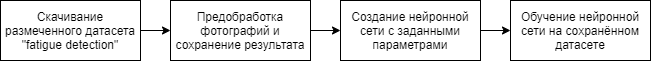
\includegraphics[width=1\linewidth]{ResNet_train.png}
        \caption{Общий процесс обучения нейронной сети}
        \label{fig:ResNet_train}
    \end{figure}
    
    \begin{figure}[H]
        \centering
        
\includegraphics[width=1\linewidth]{ResNet_use.png}
        \caption{Процесс использования нейронной сети}
        \label{fig:ResNet_use}
    \end{figure}

    Нейросеть обучалась максимум до 100 эпох с использованием критерия ранней остановки равным 10 эпохам: если в течение них минимальное значение функции потерь на валидационных данных не уменьшалось, то обучение останавливалось. В добавок было использовано уменьшение скорости обучения - если при 5 эпохах значение потерь валидационных данных слабо уменьшалось, то скорость обучения снижалась в 5 раз.
    
\section{Обоснование}\label{sec:justification}

    Использование CNN мотивировано специализированностью нейросетей данной архитектуры на обработке изображений. Не нужно выделять признаки вручную; инвариантность для сдвигов и искажений; учитываются структурные особенности изображения; общие веса позволяют снизить их количество; меньшее, по сравнению с полносвязной нейронной сетью, количество связей между нейронами увеличивает производительность системы.\cite{bengio_convolutional_1997}
    
    Рассмотренные выше существующие решения обладают рядом особенностей, которые снижают для нас ценность использования их решений к минимуму. Например, предложенные автомобильные системы по распознаванию усталости водителей имеют существенное ограничение, используя такие данные как положение руля или шаблоны езды. Система <<PERCLOS>>, обнаруживающая сонливость, путем отслеживания положения век имеет достаточно спорную надежность и предполагает сбор данных в течение длительного времени. Для нас критично иметь программное решение, обладающее достаточно надежной степенью определения усталости в условиях высокой скоростью распознавания, ограничения на число изображений и открытого доступа к исходному коду.
    
    На основе сравнения существующих решений выше и особенностей предложенной нами архитектуры проекта, можно обозначить как предполагаемые достоинства, так и недостатки представленного нами решения. 

    Разработанное решение имеет достаточно неплохую точность (accuracy - 87\%). Главным его достоинством можно выделить наличие исходного кода программной системы в открытом доступе, доступным для использования, модификации и обновления для всех желающих.
    
\section{Результаты}\label{sec:validation}


\subsection{Варианты предобработки}
    Первоначально для нормирования входных фотографий использовалась библиотека OpenCV для предобработки входных данных (фотографий). На первом этапе определялось расположение лица и глаз по признакам Хаара. По координатам глаз происходило горизонтальное выравнивание и обрезалась лишняя часть без лица. Разрешение изображения масштабировалось до 250 пикселей с каждой стороны.
    
    В ходе тестирования выяснилось, что фотографии не всегда выравниваются корректно. Для решения этой проблемы было использовано стороннее решение с применением библиотеки dlib. Такое решение лучше определяет расположение лиц, но не выравнивает лица по глазам, что нивелируется новым датасетом, в котором фотографии уже выровнены. Использование такого варианта хорошо сказалось на результатах и повысило точность с 70\% до 87\%.


\subsection{Эксперименты с датасетом LFW}

    Изначально для обучения и тестирования нейросети был выбран датасет LFW \cite{kawulok_advances_2016}. Он содержит около 13 тысяч нормализованных неразмеченных изображений лиц разных людей, что вызвало необходимость разработать сервис для разметки фотографий вручную. Фотографии разделялись на 6 классов степеней усталости: от 0\% до 100\% с шагом в 20\%.
    
    Данный сервис \cite{bairamovazat_bairamovazatneuralsetstorage_2021} представлял из себя веб-приложение, которое позволяло загружать не размеченные изображения и после оценивать их. Весь результат можно скачать архивом для дальнейшей работы с уже размеченным датасетом.
    
    \begin{figure}[H]
        \centering
        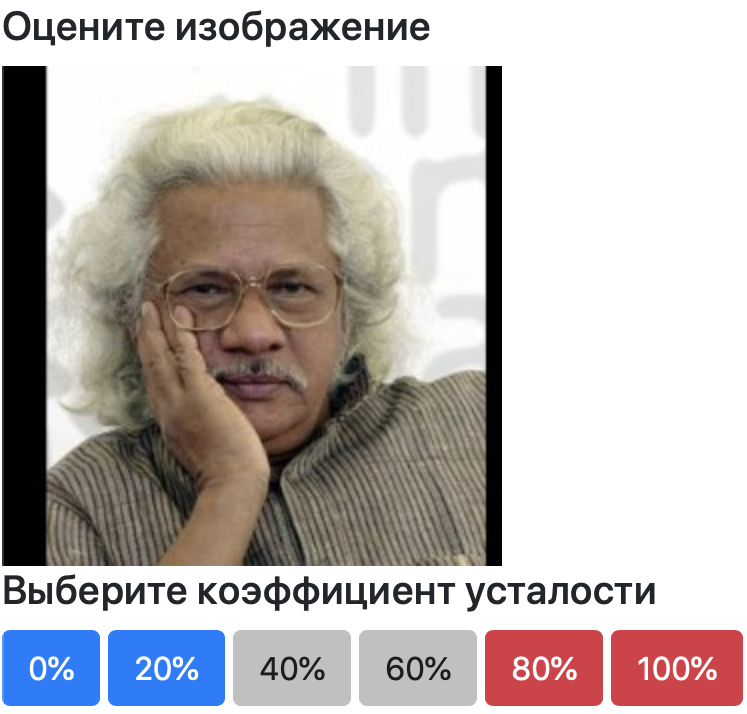
\includegraphics[width=1\linewidth]{test_man.png}
        \caption{Пример оценки изображения}
        \label{fig:test_man}
    \end{figure}

    Как показали результаты обучения, качество разметки было неудовлетворительным, и нам не удалось достигнуть приемлемых результатов точности на проверочной выборке, что отображено на рисунке \ref{fig:old_dataset_result}. К недостаткам данного датасета также можно отнести малое количество изображений критически усталых людей, обнаружение которых является критичным в условиях реальной эксплуатации.
    
    \begin{figure}[H]
        \centering
        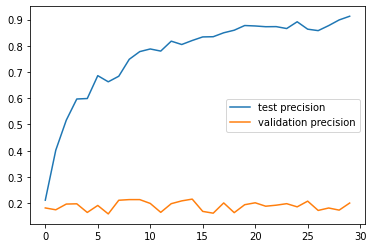
\includegraphics[width=1\linewidth]{old_dataset_results.png}
        \caption{Результаты обучения нейросети на самодельном датасете, ось абсцисс - количество эпох, ось ординат - показатель точности}
        \label{fig:old_dataset_result}
    \end{figure}
    
    На рисунке \ref{fig:old_dataset_result} показаны конечные результаты точности данного эксперимента. По горизонтальной оси указано количество эпох, по вертикальной - точность распознавания усталости, оранжевая и синяя линии - тренировочная и валидационная выборка фотографий соответственно.
    
    Как мы можем увидеть, валидационная выборка достигла точности определения усталости - 20\%, что является слабым результатом и мало отличается от статистической погрешности в 16.7\%. В последствии, было принято решение сменить датасет.
    
    
\subsection{Эксперименты с датасетом ''fatigue detection''}
    
    Нейронная сеть на базе ResNet-152v2 была обучена на выборке, состоящей из 3 513 размеченных фотографий. Эксперимент проводился на тестовой выборке размером в 394 фотографии.

    \begin{figure}[H]
        \centering
        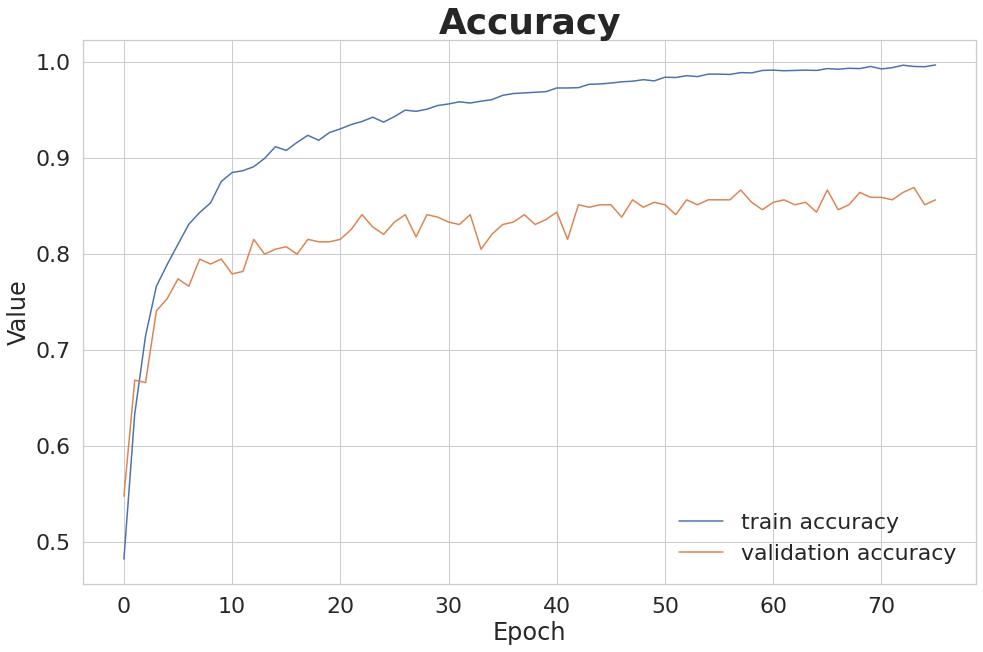
\includegraphics[width=1\linewidth]{accuracy.png}
        \caption{Результаты точности (accuracy) на тренировочной и валидационной выборках после обучения}
        \label{fig:accuracy}
    \end{figure}
    
    На рисунке \ref{fig:accuracy} показаны конечные результаты точности данного эксперимента. По горизонтальной линии указано количество эпох, по вертикальной - точность распознавания усталости, оранжевая и синяя линии - тренировочная и валидационная выборка фотографий соответственно. Как мы можем увидеть, валидационная выборка имеет лучшую точность определения усталости - 0.87, что является хорошим результатом.
    
    \begin{figure}[H]
        \centering
        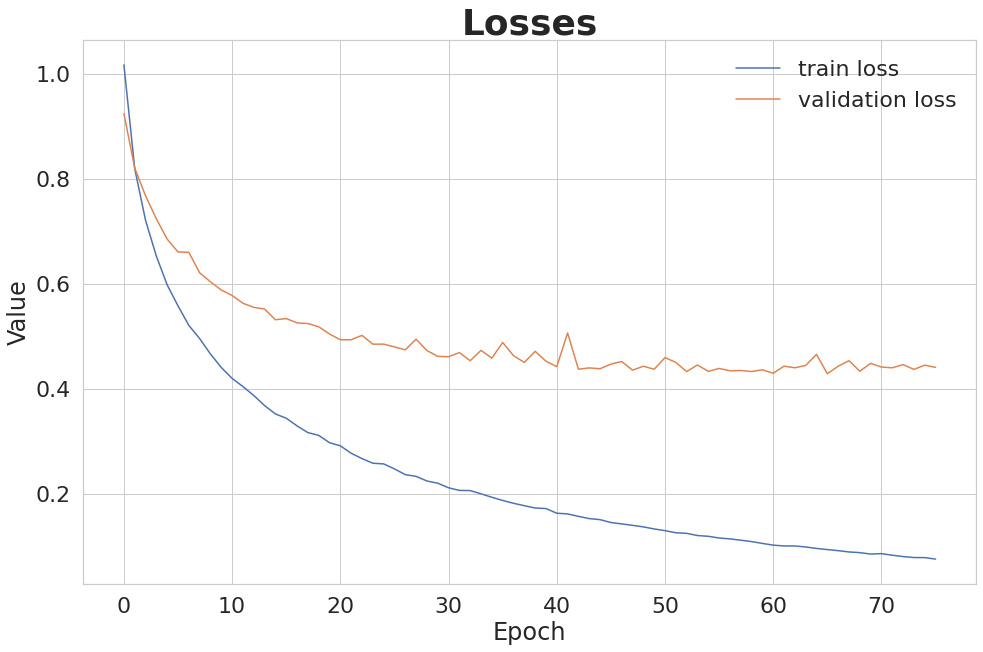
\includegraphics[width=1\linewidth]{losses.png}
        \caption{Результаты ошибки на тренировочной и валидационной выборках после обучения}
        \label{fig:losses}
    \end{figure}
     
     На рисунке \ref{fig:losses} изображены изменения ошибки в процессе обучения. Как видно на графике, на валидационных данных значение ошибки перестает существенно изменяться на 50 эпохе.
    
    \begin{figure}[H]
        \centering
        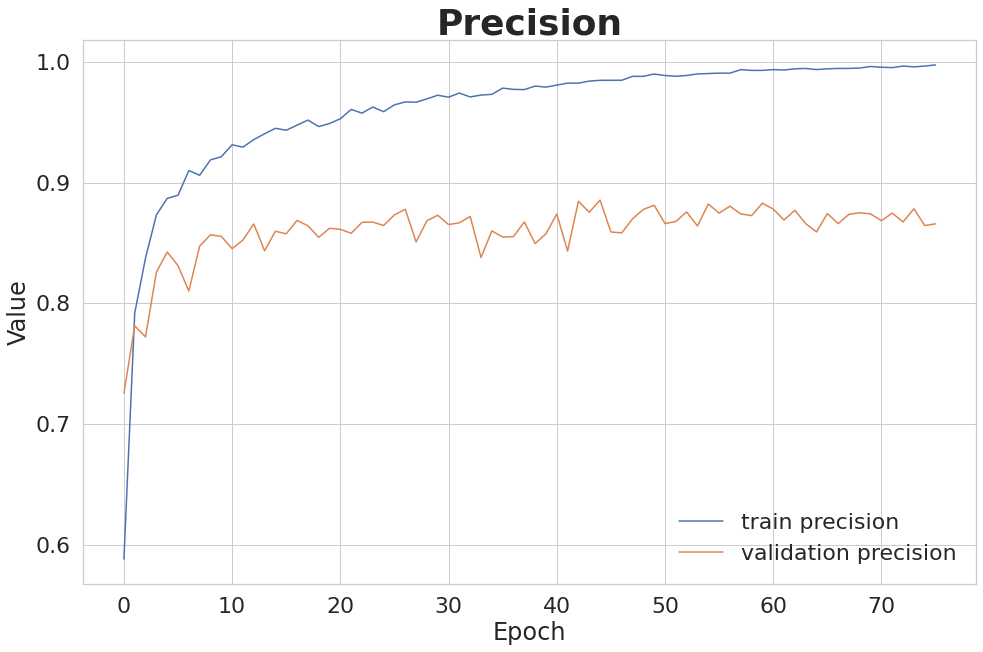
\includegraphics[width=1\linewidth]{precision.png}
        \caption{Результаты точности (precision) на тренировочной и валидационной выборках после обучения}
        \label{fig:precision}
    \end{figure}
    
    На рисунке \ref{fig:precision} показаны результаты точности (precision) валидационной выборки после обучения. По графику можно заметить, что с увеличением количества эпох точность распознавания усталости растет и достигает 0.88 на лучшей эпохе.
 
\section{Заключение}\label{sec:conclusion}

    В этой статье были описаны решения проблемы распознавания усталости человека по изображению его лица.
    В ходе данной работы были рассмотрены уже существующие алгоритмы, а также была предложена и разработана собственная модель нейронной сети определяющая усталость человека по фотографии на основе модели сверточной сети ResNet-152v2. Точности accuracy и precision составили около 87\% и 88\% соответственно у модели на лучшей эпохе.
    
    В рамках последующих работ планируется научить нейросеть определять степень усталости человека по видео в режиме реального времени, что существенно расширит возможности использования данного решения. 
 
\printbibliography
    
\end{document}